\section{Шифрование открытого текста на основе эллиптических кривых}

Цель работы  - зашифровать открытый текст, используя алфавит, приведённый в учебно-методическом пособии к выполнению лабораторного практикума по дисциплине <<Криптография>> в подразделе <<Задачи к лабораторным работам по криптографии на эллиптических кривых (используется кривая $E751( -1,1)$ − и генерирующая точка $G = (0, 1)$)>>.

\begin{table}[H]
	\centering
	\begin{tabular}{|c|c|}
		\hline
		Номер варианта                                                                                  & 7                               \\ \hline
		Открытый текст                                                                                  & терпеливо                       \\ \hline
		Открытый ключ B                                                                                 & (725, 195)                      \\ \hline
		\begin{tabular}[c]{@{}c@{}}Значения случайных чисел k для\\ букв открытого текста\end{tabular} & 17, 5, 4, 17, 13, 2, 17, 14, 19 \\ \hline
	\end{tabular}
\end{table}

Пользователь $A$ решил передать пользователю $B$ сообщение <<\textbf{терпеливо}>>. В нашем алфавите эти буквы кодируются как представлено в таблице \ref{tbl1}.

\begin{table}[H]
	\centering
	\caption{Кодирование заданного сообщения}
	\begin{tabular}{|c|c|}
		\hline
		Символ & Точка      \\ \hline
		т      & (247, 266) \\ \hline
		е      & (234, 587) \\ \hline
		р      & (243, 87)  \\ \hline
		п      & (240, 442) \\ \hline
		е      & (234, 587) \\ \hline
		л      & (237, 454) \\ \hline
		и      & (236, 39)  \\ \hline
		в      & (229, 151) \\ \hline
		о      & (240, 309) \\ \hline
	\end{tabular}
	\label{tbl1}
\end{table}

Для заданий лабораторной работы выбрана кривая E751 (−1,1) , т.е. $y^2 = x^3 − x +1 \pmod{751}$. Кривая представлена на рисунке \ref{fig:elcurve3}.

\begin{figure}[H]
	\centering
	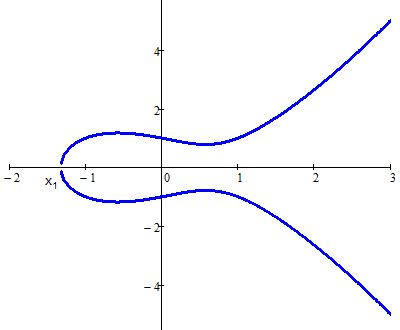
\includegraphics[width=0.7\linewidth]{img/elCurve3}
	\caption{Кривая $y^2 = x^3 − x +1$}
	\label{fig:elcurve3}
\end{figure}


Шифрованный текст имеет вид $C_m = \{ kG, P_m + k \cdot P_b\}$.

Для нахождения $kG$ используем правила сложения точек эллиптической кривой.
\[
x_3 = \lambda^2 - x_1 - x_2 \pmod{p} 
\]

\[
y_3 = \lambda(x_1-x_3) -y_1 \pmod{p}
\]


\[
\lambda = 
\begin{cases}
\frac{y_2-y_1}{x_2-x_1}, & P \neq Q\\
\frac{3x^2_1+a}{2y_1}, & P = Q
\end{cases}
\]



Вычисляем 2G:

\[
\lambda = \frac{ 3 \cdot 0^2 + (-1) }{2 \cdot 1} = \frac{-1}{2} = -1 \cdot 2^{-1} = 750 \cdot 376\mod{751} = 375\mod{751}
\]


\[
x = 375^2 - 0 - 0 \mod{751} = 188\mod{751}
\]


\[
y = 375 \cdot (0 - 188) - 1\mod{751} = 93\mod{751}
\]

\textbf{2G = (188, 93)}

Вычисляем 3G:

\[
\lambda = \frac{1-93}{0-188} = \frac{-92}{-188} = 92 \cdot 188^{-1}\mod{751} = 92 \cdot 4\mod{751}
\]


\[
x = 368^2 - 188 - 0 \mod{751} = 56\mod{751}
\]


\[
y = 368 \cdot (188 - 56) - 93\mod{751} = 419\mod{751}
\]

\textbf{3G = (56, 419)}

Вычисляем 4G:

\[
\lambda = \frac{ 3 \cdot 188^2 + (-1) }{2 \cdot 93} = \frac{106031}{186} = 106031 \cdot 186^{-1} = 140 \cdot 214\mod{751} = 671\mod{751}
\]


\[
x = 671^2 - 188 - 188 \mod{751} = 16\mod{751}
\]


\[
y = 671 \cdot (188 - 16) - 93\mod{751} = 416\mod{751}
\]

\textbf{4G = (16, 416)}

Вычисляем 5G:

\[
\lambda = \frac{93-419}{188-56} = \frac{-326}{132} = -326 \cdot 132^{-1}\mod{751} = 425 \cdot 165\mod{751}
\]


\[
x = 282^2 - 56 - 188 \mod{751} = 425\mod{751}
\]


\[
y = 282 \cdot (56 - 425) - 419\mod{751} = 663\mod{751}
\]

\textbf{5G = (425, 663)}

Вычисляем 6G:

\[
\lambda = \frac{ 3 \cdot 56^2 + (-1) }{2 \cdot 419} = \frac{9407}{838} = 9407 \cdot 838^{-1} = 395 \cdot 587\mod{751} = 557\mod{751}
\]


\[
x = 557^2 - 56 - 56 \mod{751} = 725\mod{751}
\]


\[
y = 557 \cdot (56 - 725) - 419\mod{751} = 195\mod{751}
\]

\textbf{6G = (725, 195)}

Вычисляем 7G:

\[
\lambda = \frac{419-416}{56-16} = \frac{3}{40} = 3 \cdot 40^{-1}\mod{751} = 3 \cdot 169\mod{751}
\]


\[
x = 507^2 - 16 - 56 \mod{751} = 135\mod{751}
\]


\[
y = 507 \cdot (16 - 135) - 416\mod{751} = 82\mod{751}
\]

\textbf{7G = (135, 82)}

Вычисляем 8G:

\[
\lambda = \frac{ 3 \cdot 16^2 + (-1) }{2 \cdot 416} = \frac{767}{832} = 767 \cdot 832^{-1} = 16 \cdot 102\mod{751} = 130\mod{751}
\]


\[
x = 130^2 - 16 - 16 \mod{751} = 346\mod{751}
\]


\[
y = 130 \cdot (16 - 346) - 416\mod{751} = 242\mod{751}
\]

\textbf{8G = (346, 242)}

Вычисляем 9G:

\[
\lambda = \frac{416-663}{16-425} = \frac{-247}{-409} = 247 \cdot 409^{-1}\mod{751} = 247 \cdot 213\mod{751}
\]


\[
x = 41^2 - 425 - 16 \mod{751} = 489\mod{751}
\]


\[
y = 41 \cdot (425 - 489) - 663\mod{751} = 468\mod{751}
\]

\textbf{9G = (489, 468)}

Вычисляем 10G:

\[
\lambda = \frac{ 3 \cdot 425^2 + (-1) }{2 \cdot 663} = \frac{541874}{1326} = 541874 \cdot 1326^{-1} = 403 \cdot 64\mod{751} = 258\mod{751}
\]


\[
x = 258^2 - 425 - 425 \mod{751} = 377\mod{751}
\]


\[
y = 258 \cdot (425 - 377) - 663\mod{751} = 456\mod{751}
\]

\textbf{10G = (377, 456)}

Вычисляем 11G:

\[
\lambda = \frac{1-456}{0-377} = \frac{-455}{-377} = 455 \cdot 377^{-1}\mod{751} = 455 \cdot 251\mod{751}
\]


\[
x = 53^2 - 377 - 0 \mod{751} = 179\mod{751}
\]


\[
y = 53 \cdot (377 - 179) - 456\mod{751} = 275\mod{751}
\]

\textbf{11G = (179, 275)}

Вычисляем 12G:

\[
\lambda = \frac{ 3 \cdot 725^2 + (-1) }{2 \cdot 195} = \frac{1576874}{390} = 1576874 \cdot 390^{-1} = 525 \cdot 518\mod{751} = 88\mod{751}
\]


\[
x = 88^2 - 725 - 725 \mod{751} = 286\mod{751}
\]


\[
y = 88 \cdot (725 - 286) - 195\mod{751} = 136\mod{751}
\]

\textbf{12G = (286, 136)}

Вычисляем 13G:

\[
\lambda = \frac{195-82}{725-135} = \frac{113}{590} = 113 \cdot 590^{-1}\mod{751} = 113 \cdot 737\mod{751}
\]


\[
x = 671^2 - 135 - 725 \mod{751} = 283\mod{751}
\]


\[
y = 671 \cdot (135 - 283) - 82\mod{751} = 493\mod{751}
\]

\textbf{13G = (283, 493)}

Вычисляем 14G:

\[
\lambda = \frac{ 3 \cdot 135^2 + (-1) }{2 \cdot 82} = \frac{54674}{164} = 54674 \cdot 164^{-1} = 602 \cdot 664\mod{751} = 196\mod{751}
\]


\[
x = 196^2 - 135 - 135 \mod{751} = 596\mod{751}
\]


\[
y = 196 \cdot (135 - 596) - 82\mod{751} = 433\mod{751}
\]

\textbf{14G = (596, 433)}

Вычисляем 15G:

\[
\lambda = \frac{82-242}{135-346} = \frac{-160}{-211} = 160 \cdot 211^{-1}\mod{751} = 160 \cdot 210\mod{751}
\]


\[
x = 556^2 - 346 - 135 \mod{751} = 745\mod{751}
\]


\[
y = 556 \cdot (346 - 745) - 242\mod{751} = 210\mod{751}
\]

\textbf{15G = (745, 210)}

Вычисляем 16G:

\[
\lambda = \frac{ 3 \cdot 346^2 + (-1) }{2 \cdot 242} = \frac{359147}{484} = 359147 \cdot 484^{-1} = 169 \cdot 45\mod{751} = 95\mod{751}
\]


\[
x = 95^2 - 346 - 346 \mod{751} = 72\mod{751}
\]


\[
y = 95 \cdot (346 - 72) - 242\mod{751} = 254\mod{751}
\]

\textbf{16G = (72, 254)}

Вычисляем 17G:

\[
\lambda = \frac{242-468}{346-489} = \frac{-226}{-143} = 226 \cdot 143^{-1}\mod{751} = 226 \cdot 730\mod{751}
\]


\[
x = 511^2 - 489 - 346 \mod{751} = 440\mod{751}
\]


\[
y = 511 \cdot (489 - 440) - 468\mod{751} = 539\mod{751}
\]

\textbf{17G = (440, 539)}

Вычисляем 18G:

\[
\lambda = \frac{ 3 \cdot 489^2 + (-1) }{2 \cdot 468} = \frac{717362}{936} = 717362 \cdot 936^{-1} = 157 \cdot 341\mod{751} = 216\mod{751}
\]


\[
x = 216^2 - 489 - 489 \mod{751} = 618\mod{751}
\]


\[
y = 216 \cdot (489 - 618) - 468\mod{751} = 206\mod{751}
\]

\textbf{18G = (618, 206)}

Вычисляем 19G:

\[
\lambda = \frac{468-456}{489-377} = \frac{12}{112} = 12 \cdot 112^{-1}\mod{751} = 12 \cdot 114\mod{751}
\]


\[
x = 617^2 - 377 - 489 \mod{751} = 568\mod{751}
\]


\[
y = 617 \cdot (377 - 568) - 456\mod{751} = 355\mod{751}
\]

\textbf{19G = (568, 355)}

Вычисляем $Pm+kPb$ для каждой буквы в слове.

\textbf{$Pm(\text{т})+k \cdot Pb = (247, 266) + 17 \cdot (725, 195) = (247, 266) + (179, 275) = (663, 275)$}

\[
\lambda = \frac{275-266}{179-247} = \frac{9}{-68} = 9 \cdot -68^{-1}\mod{751} = 9 \cdot 254\mod{751}
\]


\[
x = 33^2 - 247 - 179 \mod{751} = 663\mod{751}
\]


\[
y = 33 \cdot (247 - 663) - 266\mod{751} = 275\mod{751}
\]

\textbf{$Pm(\text{е})+k \cdot Pb = (234, 587) + 5 \cdot (725, 195) = (234, 587) + (1, 1) = (638, 131)$}

\[
\lambda = \frac{1-587}{1-234} = \frac{-586}{-233} = 586 \cdot 233^{-1}\mod{751} = 586 \cdot 361\mod{751}
\]


\[
x = 515^2 - 234 - 1 \mod{751} = 638\mod{751}
\]


\[
y = 515 \cdot (234 - 638) - 587\mod{751} = 131\mod{751}
\]

\textbf{$Pm(\text{р})+k \cdot Pb = (243, 87) + 4 \cdot (725, 195) = (243, 87) + (327, 108) = (228, 480)$}

\[
\lambda = \frac{108-87}{327-243} = \frac{21}{84} = 21 \cdot 84^{-1}\mod{751} = 21 \cdot 152\mod{751}
\]


\[
x = 188^2 - 243 - 327 \mod{751} = 228\mod{751}
\]


\[
y = 188 \cdot (243 - 228) - 87\mod{751} = 480\mod{751}
\]

\textbf{$Pm(\text{п})+k \cdot Pb = (240, 442) + 17 \cdot (725, 195) = (240, 442) + (179, 275) = (329, 447)$}

\[
\lambda = \frac{275-442}{179-240} = \frac{-167}{-61} = 167 \cdot 61^{-1}\mod{751} = 167 \cdot 197\mod{751}
\]


\[
x = 606^2 - 240 - 179 \mod{751} = 329\mod{751}
\]


\[
y = 606 \cdot (240 - 329) - 442\mod{751} = 447\mod{751}
\]

\textbf{$Pm(\text{е})+k \cdot Pb = (234, 587) + 13 \cdot (725, 195) = (234, 587) + (283, 258) = (463, 736)$}

\[
\lambda = \frac{258-587}{283-234} = \frac{-329}{49} = -329 \cdot 49^{-1}\mod{751} = 422 \cdot 46\mod{751}
\]


\[
x = 637^2 - 234 - 283 \mod{751} = 463\mod{751}
\]


\[
y = 637 \cdot (234 - 463) - 587\mod{751} = 736\mod{751}
\]

\textbf{$Pm(\text{л})+k \cdot Pb = (237, 454) + 2 \cdot (725, 195) = (237, 454) + (286, 136) = (688, 741)$}

\[
\lambda = \frac{136-454}{286-237} = \frac{-318}{49} = -318 \cdot 49^{-1}\mod{751} = 433 \cdot 46\mod{751}
\]


\[
x = 392^2 - 237 - 286 \mod{751} = 688\mod{751}
\]


\[
y = 392 \cdot (237 - 688) - 454\mod{751} = 741\mod{751}
\]

\textbf{$Pm(\text{и})+k \cdot Pb = (236, 39) + 17 \cdot (725, 195) = (236, 39) + (179, 275) = (407, 669)$}

\[
\lambda = \frac{275-39}{179-236} = \frac{236}{-57} = 236 \cdot -57^{-1}\mod{751} = 236 \cdot 527\mod{751}
\]


\[
x = 457^2 - 236 - 179 \mod{751} = 407\mod{751}
\]


\[
y = 457 \cdot (236 - 407) - 39\mod{751} = 669\mod{751}
\]

\textbf{$Pm(\text{в})+k \cdot Pb = (229, 151) + 14 \cdot (725, 195) = (229, 151) + (135, 669) = (6, 218)$}

\[
\lambda = \frac{669-151}{135-229} = \frac{518}{-94} = 518 \cdot -94^{-1}\mod{751} = 518 \cdot 743\mod{751}
\]


\[
x = 362^2 - 229 - 135 \mod{751} = 6\mod{751}
\]


\[
y = 362 \cdot (229 - 6) - 151\mod{751} = 218\mod{751}
\]

\textbf{$Pm(\text{о})+k \cdot Pb = (240, 309) + 19 \cdot (725, 195) = (240, 309) + (591, 555) = (561, 140)$}

\[
\lambda = \frac{555-309}{591-240} = \frac{246}{351} = 246 \cdot 351^{-1}\mod{751} = 246 \cdot 659\mod{751}
\]


\[
x = 649^2 - 240 - 591 \mod{751} = 561\mod{751}
\]


\[
y = 649 \cdot (240 - 561) - 309\mod{751} = 140\mod{751}
\]

\textbf{Итог шифрования:}

$Cm(\text{т})$ = ((440, 539), (663, 275))

$Cm(\text{е})$ = ((425, 663), (638, 131))

$Cm(\text{р})$ = ((16, 416), (228, 480))

$Cm(\text{п})$ = ((440, 539), (329, 447))

$Cm(\text{е})$ = ((283, 493), (463, 736))

$Cm(\text{л})$ = ((188, 93), (688, 741))

$Cm(\text{и})$ = ((440, 539), (407, 669))

$Cm(\text{в})$ = ((596, 433), (6, 218))

$Cm(\text{о})$ = ((568, 355), (561, 140))

